%%%%%%%%%%%%%%%%%%% Metrics %%%%%%%%%%%%%%%%%%%
In the following each sample $D_t = (X^{(t)}, y^{(t)})$ is divided into a training split $D_t^{(train)} = (X^{(t)}_{(train)}, y^{(t)}_{(train)})$ and a testing split $D_t^{(test)} = (X^{(t)}_{(test)}, y^{(t)}_{(test)})$. The chosen splitting method is arbitrary. The training process for each sample will be conducted with $D_t^{(train)}$ and evaluation with $D_t^{(test)}$.

\citeauthor{lopezpaz2022gradientepisodicmemorycontinual} \cite{lopezpaz2022gradientepisodicmemorycontinual} come up with three different measures for model predictability, stability and plasticity. I will focus on their dynamic forms given by \citeauthor{díazrodríguez2018dontforgetforgettingnew} \cite{díazrodríguez2018dontforgetforgettingnew}, because they have been adapted for in training use, i.e. they represent a model's current state after the $t$-th training step.

\textit{Accuracy} $\mathbf{A}$ represents a models performance i.e. how well the predictions $\hat{y}^{(t)}_{(test)}$ align with the true values of $y^{(t)}_{(test)}$ for a metric $\mu$ . When $A_{i,k} = \mu(\hat{y}_{(test)}^{(k)}, y_{(test)}^{(k)}) \in [0,1]$ is the accuracy measured on the $k$-th test split after the $i$-th training step, then
\begin{equation}
	\mathbf{A} = \frac{2}{t(t-1)}\sum_{i \geq k }^{t} A_{i,k}
\end{equation}
is the average accuracy after the $t$-th training step over all test splits $D_k^{(test)}, k <= t$.

\textit{Backward Transfer} $\mathbf{BWT}$ evaluates a models stability. The metric quantifies the influence that learning sample $D_{t+1}^{(train)}$ has on the performance over test sample $D_t^{(test)}$ \cite{lopezpaz2022gradientepisodicmemorycontinual}. Given the above mentioned individual \textit{Accuracy} scores $A_{i,k}$
\begin{equation}
	\mathbf{BWT} = \frac{2}{t(t-1)} \sum_{i=2}^{t}\sum_{k=1}^{i-1}(A_{i,k}-A_{k,k})
\end{equation}
is the average backward transfer after the $t$-th training step. Note that $\mathbf{BWT}$ can be negative. This property captures (catastrophic) forgetting \cite{LW}.

\textit{Forward Transfer} $\mathbf{FWT}$ is a metric for model plasticity. Complementary to BWT, \textit{Forward Transfer} measures how previous training steps influence the current one. Again, the individual \textit{Accuracy} scores are the basis for this evaluation metric. The average influence of old training steps on the model performance after the $t$-th step is:
\begin{equation}
	\mathbf{FWT} = \frac{2}{t(t-1)}\sum_{i < k }^{t} A_{i,k}
\end{equation}.

One of the motivations for CL is limited memory space for data which is why storing a test sample for each task is limiting in the long run when the number of tasks goes to infinity. A metric that directly measures the relationship between stability and plasticity on the model is presented by \citeauthor{mirzadeh2020understandingroletrainingregimes}\cite{mirzadeh2020understandingroletrainingregimes}. They use the maximum eigenvalue of the loss' Hessian $\lambda^{max}$ to describe the width of their approximation of the loss' minimum. They hypothesize that the \textit{wideness} of this minimum correlates with the forgetting rate of the respective model.

Given $W^{(t)*}$ and $W^{(t+1)*}$, the optimal parameters after learning the $t$-th and $(t+1)$-th task and $L_t(\cdot)$ and $L_{t+1}(\cdot)$ the corresponding loss function, \citeauthor{mirzadeh2020understandingroletrainingregimes} formulate the upper bound
\begin{equation}\label{2TA}
	F_t = L_t(W^{(t+1)*}) - L_t(W^{(t)*}) \approx \frac{1}{2}{\Delta W}^\top \nabla^2 L_t(W^{(t)*}) \Delta W \leq \frac{1}{2}\lambda_t^{max}\lVert \Delta W \rVert^2
\end{equation}
for the forgetting $F_t$ of the $t$-th task. They approximate $L_t(W^{(t+1)*})$ around $W^{(t)*}$ with a second order Taylor approximation, where $\nabla^2$ is the Hessian for $L_t$ and $\Delta W$ the difference between $W^{(t+1)*}$ and $W^{(t)*}$. They argue that the loss can be approximated this way, because of its almost convex path around the minimum, for models that have more observations per sample than parameters.

Furthermore, ${\Delta W}$ is dependent on the training process of the $(t+1)$-th task, which depends on the random sample it is trained on, so one can view the differences in parameters as a random vector that follows some distribution parameterized by the eigenvalues of $\nabla^2 L_t(W^{(t)*})$ \cite{mirzadeh2020understandingroletrainingregimes}. Controlling the distance between old and new weights, as well as $\lambda^{max}$ of subsequent tasks seems to be the key to mitigating forgetting \cite{mirzadeh2020understandingroletrainingregimes}.

%%%%%%%%%%%%%%%%%%% Figure 2 %%%%%%%%%%%%%%%%%%%
\usetikzlibrary{datavisualization.formats.functions}
\begin{figure}[h!]
	\centering
	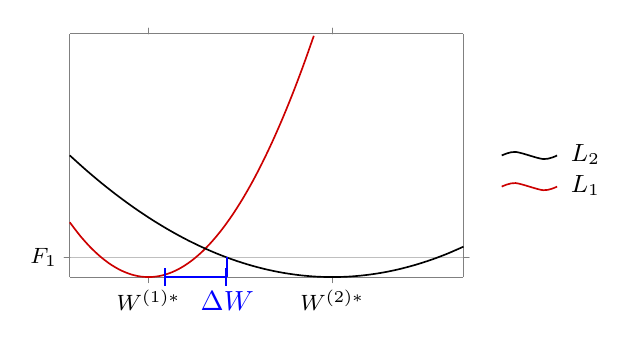
\begin{tikzpicture}[baseline]
		\datavisualization [
		scientific axes, 
		x axis = {ticks={major at={-0.2 as $W^{(1)*}$, 0.5 as $W^{(2)*}$}}},
		y axis = {max value = 0.2, ticks and grid ={major at={0.016 as $F_1$}}},
		visualize as smooth line/.list={w1,w2},
		style sheet=strong colors,
		w1 = {label in legend = {text=$L_2$}},
		w2 = {label in legend = {text=$L_1$}},
		data/format=function
		]
		data [set=w1] {
			var x : interval [-0.5:1];
			func y = 0.1 * (\value x - 0.5) * (\value x - 0.5);
		}
		data [set=w2] {
			var x : interval [-0.5:0.43];
			func y = 0.5 * (\value x  + 0.2) * (\value x + 0.2);
		};
		\usetikzlibrary{arrows.meta}
		\draw [thick, blue, |-|] (1.2, 0) -- (2, 0);
		\draw [thick, blue] (2, 0) -- (2, 0.25);
		\draw [blue] (2, -0.3) node {$\Delta W$};
	\end{tikzpicture}
	\caption{Depending on the curvature of $L_1$ and $L_2$, different $\Delta w$ result in different forgetting rates.}
	\label{fig:02}
\end{figure}